Solar radiation refers to the energy emitted by the Sun. The solar radiation received at Earth's
surface can be classified into two types: shortwave radiation with wavelengths between 0.29 and 4.0
\textmu m, and longwave radiation with wavelengths between 4 and 100 \textmu m. In the context of
photovoltaic energy generation, one is mainly concerned with shortwave radiation, as wavelengths
in the solar spectrum above 2.6 \textmu m contain very little energy.
Two terms frequently encountered in this context are irradiance and irradiation.
Irradiance, measured in \si{\watt\per\square\meter}, refers to the instantaneous flux of solar radiation
falling on any surface, while irradiation, measured in \si{\watt\hour\per\square\meter}, is the accumulated
energy flux incident on the surface over a given period of time. On its way to Earth's
surface, solar radiation interacts with atmospheric molecules. Therefore, the shortwave
solar radiation received on any surface can be divided into three components: 

\begin{itemize}
    \item \textbf{direct solar radiation \(B\)}: Solar radiation that reaches the surface without any interception
    \item \textbf{diffuse solar radiation \(D\)}: Solar radiation received after scattering and inter-reflection within the atmosphere.
    \item \textbf{reflected solar radiation \(R\)}: Solar radiation reflected from natural and human made surroundings.
\end{itemize}

\noindent
The sum of these components is termed global solar radiation (\(G\)) \cite[p. 2f]{CIBSE}.
Direct and global solar radiation are sometimes also referred to as beam and total
solar radiation, respectively. Figure \ref{fig:Radiation_components} visualizes the
three components of shortwave solar radiation.

\begin{figure}
    \centering
    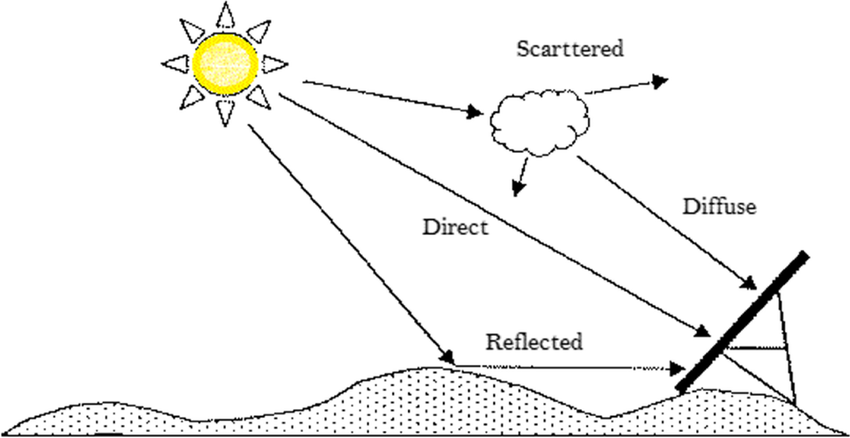
\includegraphics{Radiation_components.png}
    \caption{\small Visualization of shortwave radiation components \cite{Mghouchi}.}
    \label{fig:Radiation_components}
\end{figure}

The effect of clouds on solar radiation can be seen in Figure \ref{fig:DWD_irradiance_comparison},
which compares measured global radiation values received by a horizontally oriented surface on a
partially cloudy day with those measured on a sunny day. While the irradiance data on the sunny
day resemble a smooth haystack-shaped curve, the values on the cloudy day are much more volatile,
indicating the movement of clouds between the Sun and the measurement instrument. As clouds move
past the Sun, their edges can concentrate solar radiation and lead to short-lived spikes of up to 25 \%
increase. The spike in measured irradiance around 12:30 on the cloudy day is likely such an
occurrence \cite[p. 60]{Mayfield}.

\begin{figure}
    \centering
    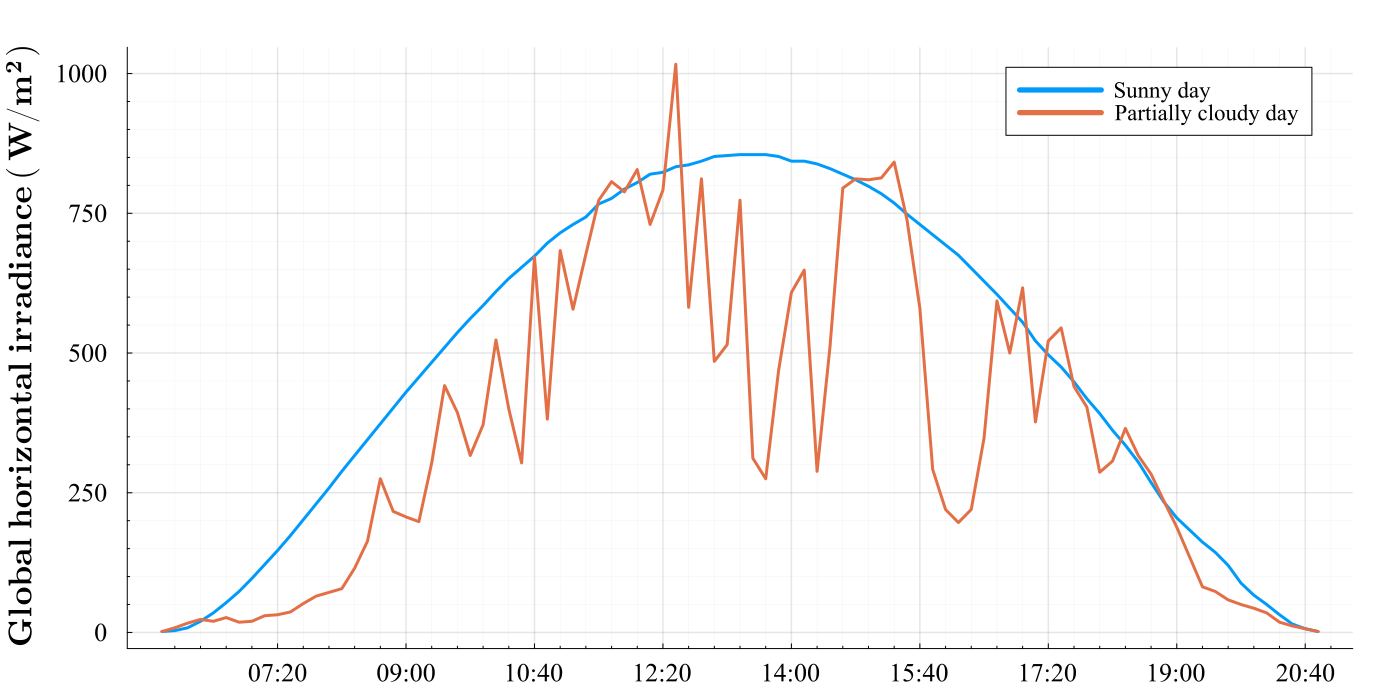
\includegraphics[scale=0.3]{DWD_irradiance_comparison.png}
    \caption{\small Global horizontal irradiance on a partially cloudy and sunny day \cite{DWD_weiherstephan_irradiance}.}
    \label{fig:DWD_irradiance_comparison}
\end{figure}

The strong influence of irradiance on photovoltaic energy generation is illustrated in Figure
\ref{fig:Surfclub_DC_output_comparison}. This figure compares the power output of a 4.62 kW
photovoltaic system on a cloudy and a sunny day, corresponding to the same days for which the
irradiance values were presented earlier. Although the photovoltaic system is not horizontally
oriented and is located approximately 18.4 km from the measurement instrument, a similar
pattern in the curves for each day is observed, indicating the well-known influence of solar
radiation on photovoltaic energy generation. It is worth mentioning that the time granularity
of the irradiance data is 10 minutes, slightly larger than the 5-minute granularity of the
photovoltaic system's production data. While the generation curve on the sunny day follows
a well-behaved approximate haystack-shaped curve, the curve on the cloudy day appears similarly
erratic. The early hours of the days provide valuable insights into irradiance values and power generation.
The PV system is shaded in the early hours due to its orientation and surrounding trees, decreasing
the amount of direct solar radiation. Interestingly, during these early hours, the measured horizontal
irradiance values on the sunny day exceed those on the cloudy day. Nevertheless, the power output in
the morning on the cloudy day is higher than on the sunny day, indicating overall more irradiance on
the PV modules due to increased diffuse radiation through clouds. This effect is confirmed by Figure
\ref{fig:DWD_diffuse_ratio}, which plots the diffuse ratio, the ratio between diffuse and global horizontal
radiation, for each of the analyzed days. The diffuse ratio on the sunny day illustrates the dominance
of direct radiation components, whereas the overcast day illustrates the contrary.

\begin{figure}
    \centering
    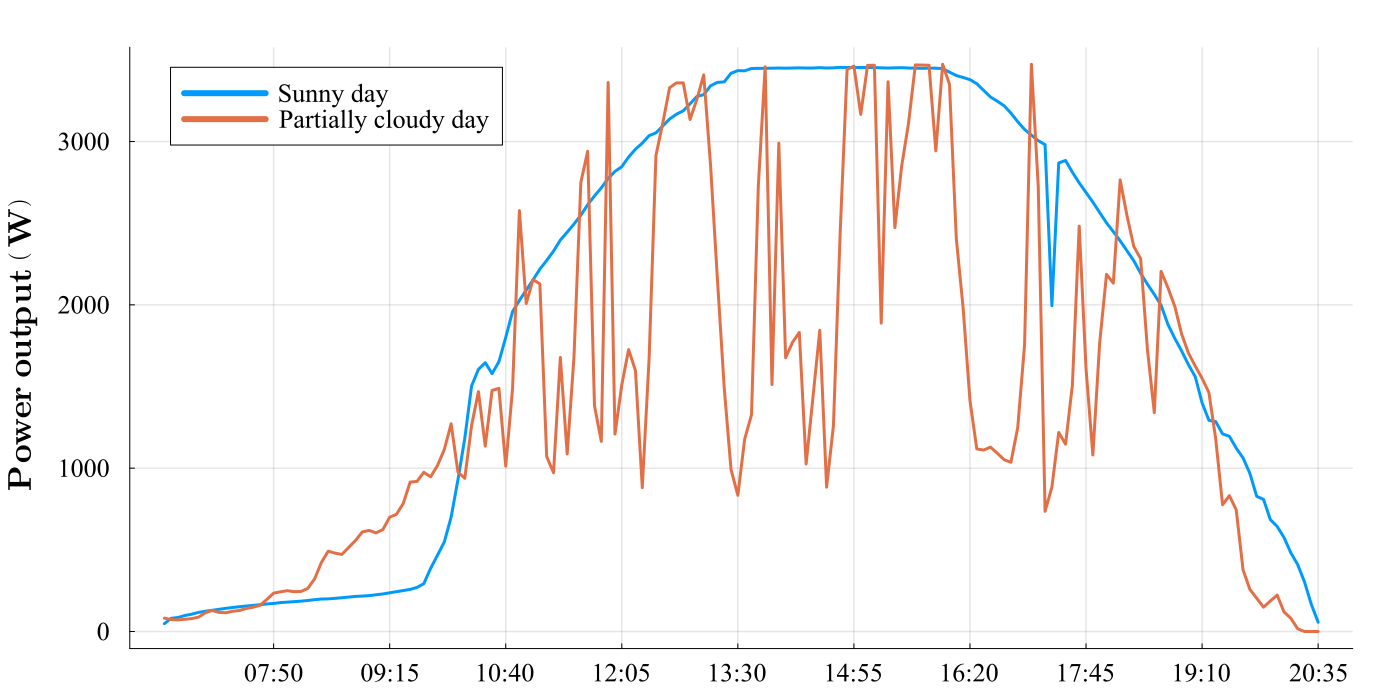
\includegraphics[scale=0.3]{Surfclub_DC_output_comparison.png}
    \caption{\small Power generation of a 4.62 kW photovoltaic system on a cloudy and sunny day.}
    \label{fig:Surfclub_DC_output_comparison}
\end{figure}

% NOTE: Kink in generation curve does not correspond to first timestamp where the solar elevation angle exceeds
% the surface tilt angle of 28°.

\begin{figure}
    \centering
    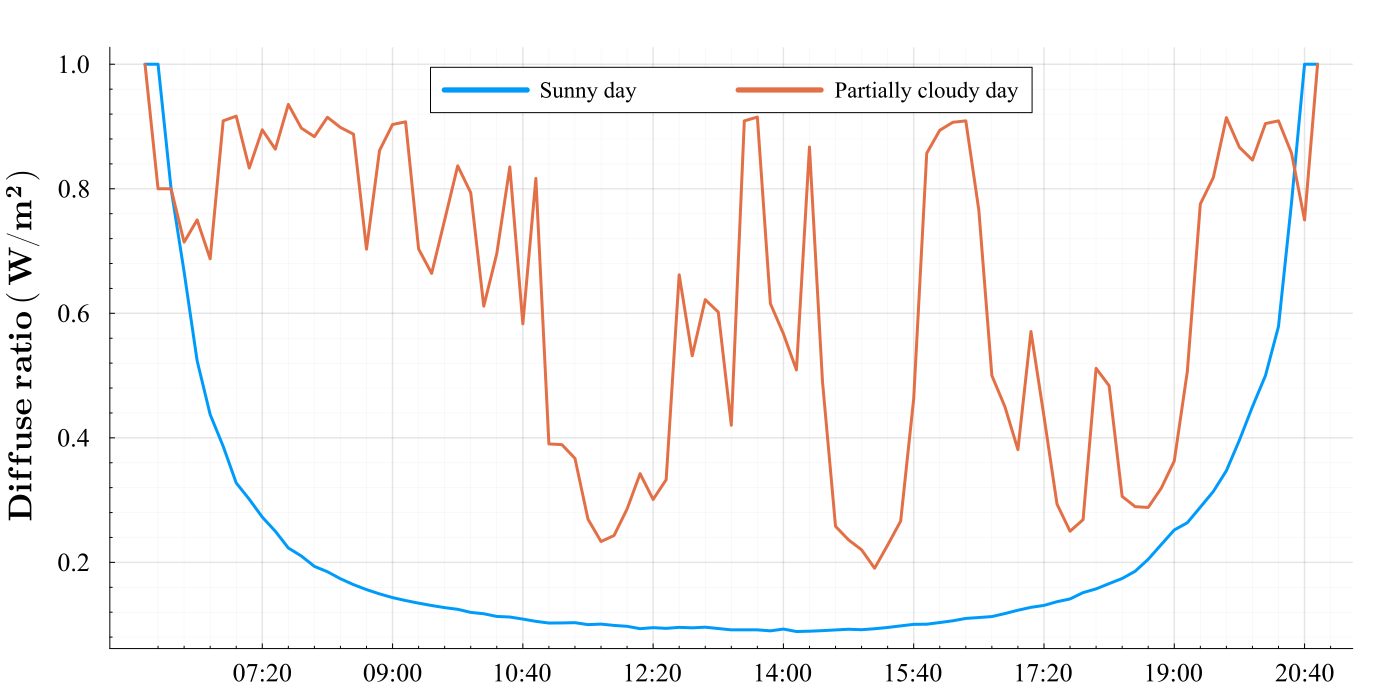
\includegraphics[scale=0.3]{DWD_diffuse_ratio.png}
    \caption{\small Comparision of diffuse ratio on a horizontal surface on a cloudy and sunny day \cite{DWD_weiherstephan_irradiance}.}
    \label{fig:DWD_diffuse_ratio}
\end{figure}